\chapter{Tworzenie REST API}
\section{Dobre praktyki}
	Interfejsy REST API są obecnie jednym z najbardziej popularnych rodzajów usług w internecie. Pozwalają różnym klientom, w tym przeglądarkom, na komunikację z serwisami sieciowymi. Bardzo ważne jest, aby prawidłowo zaprojektować REST API. Podczas tworzenia API należy wziąć pod uwagę bezpieczeństwo, wydajność oraz łatwość użycia interfejsu dla konsumentów. Z tego powodu warto poznać i stosować się do powszechnie przyjętych konwencji. W przeciwnym razie klienci oraz programiści utrzymujący projekt mogą poczuć się zdezorientowani podczas korzystania z API.
	
	W tej sekcji opisane zostanie kilka praktyk, które warto stosować przy tworzeniu REST API, aby było ono proste w użyciu oraz utrzymaniu.
	
	\subsection{Dokumentacja}
		API jest tak dobre, jak jego dokumentacja. Dokumenty opisujące działanie publicznego API powinny być dostępne publicznie i łatwo wyszukiwalne. Większość programistów sprawdzi dokumentację, zanim podejmie się jakichkolwiek prób integracji, dlatego ukrywanie jej w plikach PDF czy udostępnianie tylko po wcześniejszym zalogowaniu może zniechęcić potencjalnych klientów do korzystania z API.
		
		Dokumentacja powinna zawierać przykłady pełnych żądań i odpowiedzi. Najlepiej, aby przedstawić je w postaci możliwej do łatwego skopiowana (linki, curle lub całe zapytania, których można użyć np. w Postmanie).
		
		Po publicznym udostępnieniu API nie należy wprowadzać do niego żadnych zmian, które sprawią, że programy klientów przestaną poprawnie się z nim komunikować. Dokumentacja musi zawierać informację o poprzednich wersjach API oraz zmianach, które zostały wprowadzone.
		
		\subsubsection{Interaktywna dokumentacja}
		Interaktywna dokumentacja pozwala programistom pracować z API, dając im jasny obraz tego, jak interfejs odpowiada na żądania z różnymi parametrami i opcjami. Zapewnia wszystko, czego deweloperzy potrzebują, aby korzystać z interfejsu przy niewielkim nakładzie czasu i wysiłku. Taka dokumentacja jest niezwykle przydatna, ponieważ umożliwia testowanie, eksperymentowanie i standardowe używanie API. Przykładami narzędzi, które umożliwiają dokumentację oraz korzystanie ze stworzonego API są Postman czy Swagger.
	
	\subsection{Wersjonowanie}
		API powinno mieć określoną wersję. Dzięki temu można wprowadzać zmiany w nowszych wersjach i utrzymywać stare  wersje dla klientów, którzy nie są jeszcze gotowi do migracji ich aplikacji do nowego API. Wersja interfejsu jest najczęściej zawarta w adresie URL, aby zapewnić możliwość przeszukiwania zasobów w przeglądarce oraz ułatwia programistom pracę z API. 
		
		\begin{verbatim}
			http://www.example.com/api/v2/companies, v2 - wersja API
		\end{verbatim}
		
		Bardzo rzadko API będzie całkowicie stabilne. Ważne, aby w odpowiedni sposób informować użytkowników o zachodzących zmianach oraz utrzymywać starsze wersje API. Dobra dokumentacja i odpowiednie wersjonowanie pozwoli zapobiec wielu problemom i sprawi, że programiści będą w stanie w prosty sposób zintegrować się z API.
		
	\subsection{Sortowanie, filtrowanie i wyszukiwanie}
		Podstawowe adresy URL powinny być tak proste, jak to możliwe. Złożone filtry, żądania sortowania i zaawansowane wyszukiwanie (jeśli ograniczone do jednego zasobu) można zaimplementować jako parametry zapytania.
		\begin{enumerate}
			\item{Filtrowanie} \\
				Należy użyć unikalnego parametru zapytania dla każdego pola, które implementuje filtrowanie.
				
				\begin{verbatim}
					GET /companies?state=active 
				\end{verbatim}
				zwraca tylko aktywne firmy
				
			
			\item{Sortowanie} \\
				Podobnie jak w przypadku filtrowania, można zastosować ogólny parametr (np. sort) do opisania reguł sortowania \cite{BestPracticesWeb}. W celu bardziej złożonych operacji sortowania zezwala się na podanie listy pól oddzielonych przecinkami. Używa się '-', aby sortować malejąco względem pola.
				
				\begin{verbatim}
					GET /companies?sort=name
				\end{verbatim}
				zwraca listę firm w porządku rosnącym względem nazwy. \\
				
				\begin{verbatim}
					GET /companies?sort=-name
				\end{verbatim}
				zwraca listę firm w porządku malejącym względem nazwy. \\
			
				\begin{verbatim}
					GET /companies?sort=-amount_employees,name
				\end{verbatim}
				zwraca listę firm w porządku malejącym względem liczby pracowników, W ramach tej samej liczby pracowników sortuje firmy rosnąco względem nazwy.
					
			\item{Wyszukiwanie} \\
				Czasami podstawowe filtry i parametry sortowania nie wystarczą i potrzebne są bardziej zaawansowane wyszukiwania. Jeśli wyszukiwanie jest używane jako mechanizm pobierania zasobów, można udostępnić metodę w API z parametrem zapytania (np. query) \cite{BestPracticesWeb}. Łącząc razem wszystkie przedstawione powyżej sposoby pozyskiwania danych, można tworzyć zapytania:
				
				\begin{verbatim}
					GET /companies?state=active&sort=name
				\end{verbatim}
				
				zwraca listę aktywnych firm posortowanych po nazwie. \\
			
				\begin{verbatim}
					GET /companies/:company/notes?state=archived&sort=updated_at&query="REST API"
				\end{verbatim}
				zwraca listę notatek, które są zarchiwizowane, posortowane rosnąco po dacie ich aktualizacji oraz zawierają tekst "REST API".
				
				
				\item{Aliasy} \\
				Dobrym pomysłem jest stworzenie osobnych metod w API dla najczęściej używanych opcji wyszukiwania. Ułatwi i przyspieszy to korzystanie z API.
				
				\begin{verbatim}
					GET /companies/recently_created
				\end{verbatim}
				zwraca listę niedawno stworzonych firm.
			
		\end{enumerate}
	

	\subsection{Zwracanie zasobów}
		Użycie w zapytaniu metod POST, PATCH i PUT często powoduje zmiany w polach zasobu. Za dobrą praktykę uznaje się zwracane zaktualizowanej reprezentacji zasobu w ramach odpowiedzi.
		
		\subsubsection{Spring}
		W celu zwrócenia zasobu po aktualizacji warto wykorzystać klasę ResponseEntity wraz z pozytywnym kodem odpowiedzi HTTP oraz zasobem.
		\begin{figure}[H]
			\begin{center}
				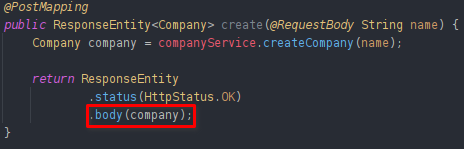
\includegraphics[scale=1.0]{spring_create_method_response.png}
				\caption{\label{fig:spring-create-company} Spring - tworzenie firmy}
			\end{center}
		\end{figure}
	
		\subsubsection{Ruby on Rails}
		W zależności od parametru format framework zwraca zasób w formacie json lub renderuje widok HTML z zasobem.
		\begin{figure}[H]
			\begin{center}
				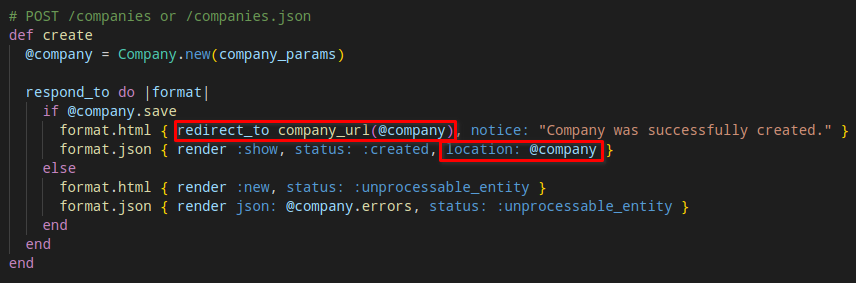
\includegraphics[scale=0.6]{ror_response.png}
				\caption{\label{fig:ror-create-company} Ruby on Rails - tworzenie firmy}
			\end{center}
		\end{figure}
	
	\subsection{JSON czy XML?}
		Współcześnie, uważa się, że XML nie jest najlepszym formatem danych w przypadku REST API. Jest zbyt szczegółowy, trudny do analizy i odczytu. Zdecydowana większość współczesnych API jest oparta o typ JSON. Format ten pożycza niektóre z dobrych stron JavaScriptu i korzysta z bezproblemowej integracji z natywnym środowiskiem przeglądarki \cite{RESTAPIDesignRulebook}. Jeśli nie istnieje jeszcze standardowy format dla danego typu zasobu (np. image/jpeg dla obrazów skompresowanych w JPEG), interfejs REST API powinien używać formatu JSON do strukturyzacji swoich informacji.
	
	\subsection{Błędy}
		Kiedy zajdzie taka potrzeba, API powinno dostarczać użytkownikowi użyteczny komunikat o błędzie w znanym formacie. Odpowiedź z błędem nie powinna różnić się strukturą od standardowych odpowiedzi (np. z aktualizowanym zasobem) \cite{BestPracticesWeb}. API w każdej odpowiedzi powinno zwracać kod statusu HTTP, aby poinformować konsumenta o stanie, w jakim znalazło się zapytania. \\
		Ciało błędów JSON powinno dostarczyć deweloperom:
		\begin{itemize}
			\item przydatny komunikat o błędzie
			\item kod błędu (który jest dokładnie opisany w dokumentacji)
			\item być może szczegółowy opis
		\end{itemize}
		\begin{figure}[H]
			\begin{center}
				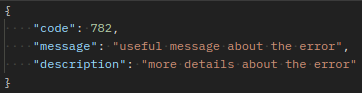
\includegraphics[scale=1.2]{error_example.png}
				\caption{\label{fig:error-message} Odpowiedź z wiadomością o błędzie}
			\end{center}
		\end{figure}
	
		Błędy walidacji dla zapytań POST, PATCH i PUT wymagają dodatkowej informacji o polach zasobu. Dobrym sposobem na poradzenie sobie z tym problemem jest użycie kodu błędu najwyższego poziomu dla błędów walidacji i dostarczenie szczegółowych błędów dla poszczególnych pól:
		\begin{figure}[H]
			\begin{center}
				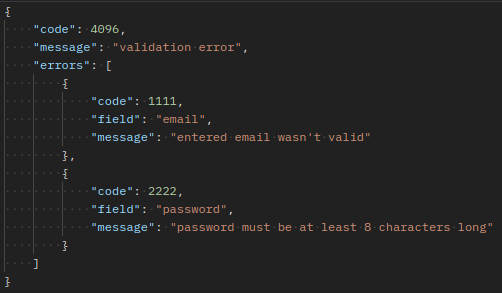
\includegraphics[scale=1.2]{error_validation_example.png}
				\caption{\label{fig:error-validation-message} Odpowiedź z wiadomością o błędzie z opisem pól}
			\end{center}
		\end{figure}
	
		\subsubsection{Ruby on Rails}
		Wygenerowany kod przy pomocy komendy
		\begin{verbatim}
			rails generate scaffold 
		\end{verbatim} 
		służący do stworzenia nowej firmy obsługuje podstawowe błędy. Metoda zwraca odpowiednią wiadomość o błędzie w zależności od przekazanego w zapytaniu parametru określającego typ danych (html/json).

		\begin{figure}[H]
			\begin{center}
				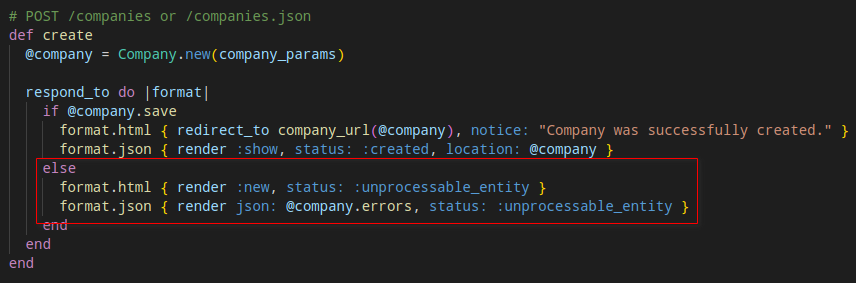
\includegraphics[scale=0.7]{ror_error_handling_ann.png}
				\caption{\label{fig:ror-create-company-error} Ruby on Rails - obsługa błędów}
			\end{center}
		\end{figure}
	
		Dla zapytania, w którym nazwa firmy jest już zajęta np.
		\begin{verbatim}
			http://localhost:3000/companies/?format=json 
			z response body {"company": {"name": "name in use"}}
		\end{verbatim}
		Aplikacja zwróci kod błędu 422 (Unprocessable Entity) wraz z informacją:
		\begin{figure}[H]
			\begin{center}
				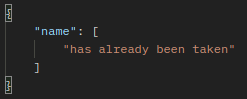
\includegraphics[scale=1.2]{ror_error_name_taken.png}
				\caption{\label{fig:ror-error-name} Ruby on Rails - odpowiedź z wiadomością o błędzie }
			\end{center}
		\end{figure}

		
		\subsubsection{Spring}
		W przypadku Springa nie można liczyć na automatycznie wygenerowany kod. Jednym ze sposobów na poradzenie sobie z obsługą błędów jest, tak jak w przypadku metody stworzonej przy pomocy komendy w Ruby on Rails obsługiwać błędy pojedynczo, ale popularnym rozwiązaniem jest zastosowanie klasy, która przechwytuje wyjątki (na poziomie kontrolera lub globalnie), a następnie zwraca odpowiednią wiadomość dla klienta \cite{SpringDocs}.
		Obsłużenie pojedynczego wyjątku może wyglądać w następujący sposób:
		\begin{figure}[H]
			\begin{center}
				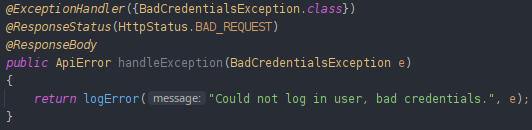
\includegraphics[scale=1.1]{spring_error_handling.png}
				\caption{\label{fig:spring-error-handling} Spring - obsługa wyjątku}
			\end{center}
		\end{figure}
	
		\noindent Z kolei odpowiedź wysłana do aplikacji klienckiej z wiadomością o błędzie może wyglądać w następujący sposób:
		\begin{figure}[H]
			\begin{center}
				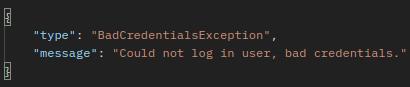
\includegraphics[scale=1.2]{spring_error_postman.png}
				\caption{\label{fig:spring-error-response} Spring - odpowiedź z wiadomością o błędzie}
			\end{center}
		\end{figure}
	
	\subsection{Testowanie}
	Warstwa API każdej aplikacji jest jednym z najbardziej kluczowych komponentów oprogramowania. Jest to kanał, który łączy klienta z serwerem (lub serwis z innym serwisem), napędza procesy biznesowe i zapewnia usługi, które dają namacalną wartość użytkownikom.
	
	Publiczny interfejs API skierowany do klienta, który jest wystawiony na działanie użytkowników końcowych, staje się produktem samym w sobie. Popsucie się go zagraża nie tylko pojedynczej aplikacji, ale całemu łańcuchowi procesów biznesowych zbudowanych wokół niej.
	
	Testy API są szybkie, upraszczają walidację logiki biznesowej, bezpieczeństwa, zgodności i innych aspektów aplikacji. W przypadku, gdy API jest publiczne i zapewnia użytkownikom końcowym programowy dostęp do aplikacji lub usług, testy API efektywnie stają się testami end-to-end i powinny obejmować pełen scenariusz użytkowania funkcjonalności.
	
	\subsubsection{Plan testowania}
	Znaczenie testów API jest oczywiste, ale co i jak powinno się testować w przypadku API? Proces testowania należy rozpocząć od testów funkcjonalnych, aby zapewnić, że interfejs działa poprawnie. Głównymi celami takiego testowania jest:
	\begin{itemize}
		\item zapewnienie, że implementacja działa poprawnie - bez błędów.
		\item zapewnienie, że implementacja działa zgodnie ze specyfikacją wymagań.
	\end{itemize}
	
	Każdy test powinien składać się z kilku punktów, które ten musi spełnić, aby zakończył się powodzeniem:
	\begin{enumerate}
		\item zweryfikowanie poprawności kodu odpowiedzi HTTP. Na przykład, niedozwolone żądanie powinno zwrócić kod 403 (Forbidden).
		\item zweryfikowanie ciała odpowiedzi, poprawności nazw pól, typów i wartości - również w odpowiedziach o błędach.
		\item zweryfikowanie nagłówków odpowiedzi, mają one wpływ zarówno na bezpieczeństwo, jak i wydajność.
		\item opcjonalnie, można sprawdzić poprawność stanu aplikacji, jeśli testy są wykonywane manualnie lub dostęp do UI jest prosty.
		\item zweryfikowanie podstawowej wydajności, jeśli operacja zakończyła się pomyślnie, ale zajęła nieuzasadnioną ilość czasu, test powinien zakończyć się niepowodzeniem.
	\end{enumerate}

	\subsubsection{Kategorie scenariuszy testowych}
	Testy można podzielić na następujące, ogólne grupy scenariuszy testowych:
	\begin{enumerate}
		\item podstawowe testy pozytywne (sprawdzają podstawową funkcjonalność i kryteria akceptacji API).
		\item rozszerzone testy pozytywne z opcjonalnymi parametrami (sprawdzają opcjonalne parametry i dodatkową funkcjonalność).
		\item negatywne testy z ważnymi danymi wejściowymi (sprawdzają, czy aplikacja obsłuży scenariusze problemowe z ważnymi danymi np. rejestracja użytkownika z e-mailem, który nie jest unikalny).
		\item negatywne testy z mniej ważnymi danymi wejściowymi (sprawdzają, czy aplikacja obsłuży scenariusze problemowe z mniej ważnymi danymi np. zmiana wieku użytkownika na wartość tekstową).
		\item testy destrukcyjne (testy, które polegają na celowym zepsuciu API w celu sprawdzenia jego stabilności).
		\item testy bezpieczeństwa, autoryzacji i uprawnień.
	\end{enumerate}
	

\section{Uwierzytelnianie i autoryzacja}
	Podczas obsługi niektórych żądań aplikacja musi wiedzieć, który użytkownik jest za nie odpowiedzialny. Uwierzytelnianie to problem powiązania żądania z użytkownikiem. Z kolei autoryzacja to problem określenia, czy użytkownik ma prawo wykonać daną akcję. Jeśli klient A chce usunąć swoje konto, trzeba mieć absolutną pewność, że to właśnie klient A jest odpowiedzialny za wywołanie akcji (jeśli ustalimy, że tylko właściciel konta może nim zarządzać).
	
	Kiedy klient API wysyła żądanie HTTP, może zawrzeć pewne dane uwierzytelniające w nagłówku HTTP Authorization. Usługa sprawdza poświadczenie i decyduje, czy poprawnie identyfikują one klienta jako konkretnego użytkownika (uwierzytelnianie), oraz czy ten użytkownik jest rzeczywiście upoważniony do zrobienia tego, o co prosi (autoryzacja). Jeśli oba warunki są spełnione, serwer realizuje żądanie \cite{RESTfulWebServices}. Jeżeli brakuje danych uwierzytelniających bądź są one niepoprawne, aby poprawnie obsłużyć żądanie, serwer wysyła komunikat z kodem 401 (Unauthorized). W przypadku kiedy klient uwierzytelnił się poprawnie, ale nie ma prawa na wykonanie akcji, serwer zwraca komunikat 403 (Forbidden).
	
	\subsection{Uwierzytelnianie}
		 
		Najpopularniejszymi sposobami na implementację uwierzytelniania są:
		\begin{itemize}
			\item{Ciasteczka sesyjne} \\
			Po pomyślnym zalogowaniu się użytkownika:
			\begin{enumerate}
				\item serwer generuje token, który jednoznacznie identyfikuje sesję użytkownika.
				\item serwer podpisuje token sekretnym kluczem.
				\item serwer wiąże token z użytkownikiem i zapisuje go w bazie.
				\item serwer wysyła ciasteczko z token do przeglądarki klienta.
				\item przeglądarka otrzymuje ciasteczko i zapisuje je lokalnie.
				\item następnie przeglądarka dołącza ciasteczko do każdego zapytania wysyłanego na serwer.
				\item dla każdego żądania serwer pobiera token z ciasteczka i porównuje go z tym, które zostało zapisane w bazie i jeśli tokeny są takie same, obsługuje żądanie.
			\end{enumerate}
			
			W podejściu opartym na ciasteczkach sesyjnych token nie zawiera żadnych informacji na temat użytkownika, jest jedynie łańcuchem losowych znaków wygenerowanych i podpisanych przez tajny klucz. Token jest zapisywany w bazie danych po stronie serwera w relacji One-to-One z użytkownikiem w celu późniejszej identyfikacji go na podstawie danych w tokenie.
		
			\item{JSON Web Token (JWT)} \\
			Po pomyślnym zalogowaniu się użytkownika:
			\begin{enumerate}
				\item serwer generuje JWT token i szyfruje go.
				\item serwer wysyła token do przeglądarki klienta.
				\item przeglądarka otrzymuje token i zapisuje go lokalnie.
				\item następnie przeglądarka dołącza token do każdego zapytania wysyłanego na serwer przy pomocy nagłówka Authorization.
				\item dla każdego żądania serwer pobiera token z nagłówka Authorization, odszyfrowuje go i wydobywa dane o użytkowniku i jego uprawnieniach. Opierając się wyłącznie na danych z tokena, jest w stanie zaakceptować lub odrzucić żądanie klienta.
			\end{enumerate}
		
			W podejściu JWT sam token jest w stanie jednoznacznie zidentyfikować użytkownika, więc token nie jest przechowywany w żadnej bazie danych po stronie serwera. Wszystkie potrzebne informacje o użytkowniku są przechowywane w tokenie JWT.
			
			\subsubsection{OAuth}
			OAuth jest otwartym protokołem, który pozwala użytkownikom zweryfikować się za pomocą zaufanego podmiotu trzeciego (Google, Microsoft Azure czy Facebook) poprzez wymianę tokenów, aby uzyskać dostęp do aplikacji. Najnowsza wersja protokołu, OAuth 2.0 jest uważana za standard w branży i wykorzystywana przez największe firmy.
			
			Największą zaletą korzystania z OAuth jest przerzucenie odpowiedzialności za zarządzanie hasłami na podmioty zewnętrzne. Zmniejsza to ilość przechowywanych danych użytkowników oraz przyśpiesza proces tworzenia aplikacji. Co więcej, użytkownicy nie potrzebują nowego konta i hasła w celu korzystania z usługi, ponieważ posługują się już istniejącym kontem. 
		\end{itemize}
	
	\subsection{Autoryzacja}
		Celem autoryzacji jest sprawdzenie, czy użytkownik jest uprawniony do korzystania z określonego zasobu (np. tylko administrator może wyświetlić stronę z listą wszystkich użytkowników serwisu). Autoryzację najczęściej implementuje się za pomocą ról. Oznacza to, że każdemu użytkownikowi jest przypisana rola (np. ADMIN, EMPLOYEE, CLIENT), którą przechowuje się w bazie danych. Następnie, dla każdego żądania, które wymaga konkretnych uprawnień, serwer sprawdza, czy klient jest upoważniony do wykonania akcji.

\section{Plan tworzenia serwisu Restful \cite{RESTfulWebServices}}
	Przed rozpoczęciem programowania REST API warto stworzyć plan, który ułatwi i ustandaryzuje proces tworzenia oprogramowania. Poniższa procedura zawiera wszystkie standardowe kroki, które należy zrealizować, aby dodać nową funkcjonalność do REST API. Trzymanie się takiego planu ułatwi deweloperom pracę z API oraz pozwoli uniknąć wielu błędów.
	
\begin{enumerate}
	\item Ustal zestaw danych.
	\item Podziel zestaw danych na zasoby. \\~\\
	Dla każdego zasobu:
	\item Nazwij zasób przy pomocy URI.
	\item Udostępnij endpointy potrzebne do korzystania z zasobu.
	\item Zaprojektuj reprezentacje zasobu przesyłaną do serwera przez klienta.
	\item Zaprojektuj reprezentacje zasobu udostępnianą dla klienta.
	\item Zintegruj nowy zasób z istniejącymi zasobami.
	\item Rozważ typowe flow związane z zasobem (co powinno się z nim stać?).
	\item Rozważ, w jakich sytuacjach mogą wystąpić błędy (co może pójść nie tak?).
\end{enumerate}

